\chapter{Análisis exploratorio de los datos}
\label{cap:eda}

En este capítulo se desarrolla el primer objetivo específico. Se describe el comportamiento de los precios mayoristas y del abastecimiento, se evalúa la calidad de los datos y se identifican los rasgos que orientan las decisiones de modelado de los capítulos siguientes.

\section{Carga de los datos y construcción del panel}
\label{sec:carga}

El SIPSA tiene dos componentes \citep{dane}. El componente de precios registra en más de 60 mercados las cotizaciones mayoristas en las horas de mayor actividad, a diario en los perecederos y semanalmente en los demás productos \citep{danefme2022}; el precio mensual es el promedio de esas cotizaciones. El componente de abastecimiento registra las toneladas que ingresan a las principales centrales y su lugar de origen. El autor construyó una base mensual que integra ambos componentes por central, producto y mes a partir de los archivos descargados del DANE (apéndice~\ref{ap:reproduccion}). Cuando el abastecimiento agrupa varias variedades de un mismo producto, como en el caso del arroz, se tomó la variedad con más meses de precio en la central. Ese conteo se hace solo con los meses hasta diciembre de 2024. En una primera versión de la base se contaron los meses de 2018 a 2025; al repetir la elección con el corte de 2024 cambió la variedad de una de las 662 combinaciones de central y producto (la panela del Mercado del Sur de Montería, que pasó de la cuadrada morena a la redonda morena) y el panel se reconstruyó con esa corrección. Todas las reglas de inclusión usan solo información hasta diciembre de 2024. Las carnes se excluyeron, ya que el abastecimiento se registra en canal y los precios corresponden a cortes. El índice ONI se obtuvo de la NOAA \citep{noaa}.

La tabla~\ref{tab:embudo} resume la construcción del panel. Se conservaron las series con precio en pesos por kilogramo y al menos 48 meses con dato hasta diciembre de 2024, criterio que no utiliza información del periodo de prueba. Además, cada observación requiere el precio del mes actual, del mes siguiente y de doce meses atrás. El panel final contiene \cfilas\ observaciones de \cseries\ series, correspondientes a \ccentrales\ centrales, \cciudades\ ciudades y \calimentos\ productos.

\begin{table}[htbp]\centering\small
\caption{De la base del SIPSA al panel de análisis. Una serie puede aparecer en varias filas, porque un mismo producto puede tener meses con y sin precio. Las carnes no se incluyen en la base unida (sección~\ref{sec:carga}).}\label{tab:embudo}
\begin{adjustbox}{max width=\textwidth}\begin{tabular}{lrr}\toprule
Paso & Registros & Series\\ \midrule
Registros de la base unida (2018--2026) & 317.322 & 5.265 \\
\quad Sin precio (solo abastecimiento) & 172.565 & 3.967 \\
\quad Precio en otra unidad (atado, docena, bulto, etc.) & 4.261 & 58 \\
Con precio en pesos por kilogramo & 140.496 & 1.777 \\
Series con al menos 48 meses con precio hasta 2024 & 123.081 & 1.260 \\
Con precio observado en $t$, $t+1$ y $t-12$ (panel) & 104.354 & 1.260 \\
\bottomrule\end{tabular}\end{adjustbox}\end{table}


Los datos se dividieron en el tiempo según el mes pronosticado (tabla~\ref{tab:muestras}). La muestra de desarrollo (febrero de 2019 a diciembre de 2024) se usó para todas las decisiones, con validación por origen móvil en 2022, 2023 y 2024: en cada año, los modelos se estiman con los meses anteriores y se evalúan en los doce meses del año. El periodo de prueba se utilizó una única vez, al final del estudio. En el resto del documento, \emph{validación} se refiere a esos tres años y \emph{entrenamiento}, al ajuste final con toda la muestra de desarrollo.

\begin{table}[htbp]\centering\small
\caption{Muestras del estudio según el mes pronosticado. Todas las decisiones usan la muestra de desarrollo, con validación por origen móvil en 2022, 2023 y 2024 (en cada año, los modelos se estiman con los meses anteriores); la prueba se evalúa una sola vez.}\label{tab:muestras}
\begin{adjustbox}{max width=\textwidth}\begin{tabular}{llrr}\toprule
Muestra & Meses pronosticados & Observaciones & Alzas mayores al 15\,\% (\%)\\ \midrule
Desarrollo & feb-2019 a dic-2024 & 80.533 & 18{,}5 \\
\quad Validación 2022 (ajuste hasta dic-2021) & ene-2022 a dic-2022 & 13.790 & 20{,}5 \\
\quad Validación 2023 (ajuste hasta dic-2022) & ene-2023 a dic-2023 & 13.588 & 16{,}1 \\
\quad Validación 2024 (ajuste hasta dic-2023) & ene-2024 a dic-2024 & 13.621 & 18{,}1 \\
Prueba & ene-2025 a sep-2026 & 23.821 & 16{,}8 \\
\bottomrule\end{tabular}\end{adjustbox}\end{table}


\section{Cobertura por central}
\label{sec:cobertura}

La tabla~\ref{tab:centrales} del apéndice describe las centrales incluidas. Las cinco de mayor tamaño aportan entre 65 y 84 series cada una, y la mayoría de las centrales tiene precio en más del 92\pct\ de los meses. Las diferencias en el cambio típico y en la frecuencia de alzas entre centrales se explican principalmente por la composición de productos. Paloquemao y Plaza Las Flores cotizan solo procesados, granos y lácteos y registran muy pocas alzas, mientras que en Tunja y Cavasa predominan los perecederos.

\section{Datos faltantes}
\label{sec:faltantes}

\subsection*{Magnitud y distribución}

Contando desde el primer mes con precio de cada serie, el \cfaltserie\pct\ de los meses no tiene precio registrado. En verduras y tubérculos la proporción de faltantes pasó de 1--2\pct\ hasta 2021 a 5--12\pct\ desde 2022, y en lácteos se encuentra la proporción más alta (figura~\ref{fig:faltantes}a). La ficha metodológica del SIPSA vigente desde 2022 \citep{danefme2022} no registra cambios en la recolección de precios, solo una actualización documental, de modo que no se pudo establecer la causa del aumento; podría deberse a la rotación de informantes o a cambios en la oferta de algunas centrales. Como el aumento coincide con la mitad del periodo de desarrollo, se incluye como una posible fuente de diferencias entre desarrollo y prueba en las limitaciones. La mayoría de los huecos son cortos (figura~\ref{fig:faltantes}b): de los \cnhuecos\ huecos identificados, el \chuecouno\pct\ dura un mes y el \chuecodos\pct\ dura dos. Los huecos de más de seis meses representan el \chuecolargo\pct\ del total, aunque concentran el \chuecomeslargo\pct\ de los meses faltantes; corresponden a series que dejaron de cotizarse temporalmente.

\begin{figure}[htbp]\centering
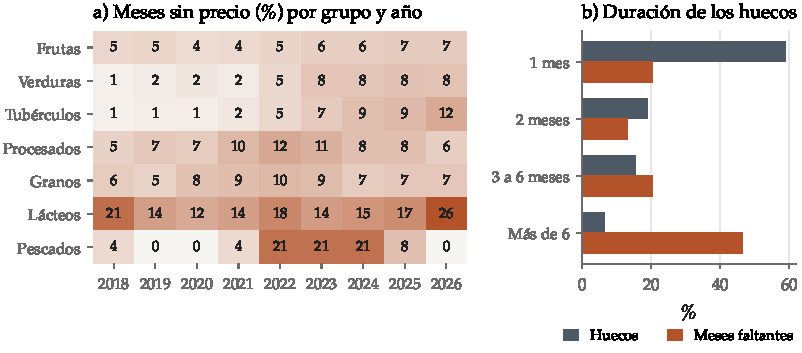
\includegraphics[width=.8\textwidth]{fig_faltantes}
\caption{(a) Porcentaje de meses sin precio por grupo y año, contando desde el primer mes con precio de cada serie. (b) Distribución de la duración de los huecos: porcentaje de huecos y porcentaje de meses faltantes que corresponden a cada duración.}\label{fig:faltantes}
\end{figure}

\subsection*{Tratamiento}

El tratamiento de los faltantes dependió del uso de cada variable (tabla~\ref{tab:falt_tratamiento}). La variable objetivo no se imputó, y las imputaciones de las variables explicativas se hicieron únicamente con información anterior al mes de pronóstico.

\begin{table}[htbp]\centering\small
\caption{Tratamiento de los datos faltantes según su uso}\label{tab:falt_tratamiento}
\begin{tabular}{>{\raggedright\arraybackslash}p{3cm}>{\raggedright\arraybackslash}p{5.1cm}>{\raggedright\arraybackslash}p{4.7cm}}\toprule
Uso & Tratamiento & Razón\\ \midrule
Variable objetivo & Solo precios observados; si falta $p_{t+1}$ la observación se excluye & Una imputación generaría cambios de precio no observados\\
Variables de precio & Se repite el último precio en huecos de hasta dos meses; si el hueco es más largo, la variable queda faltante & El 78\pct\ de los huecos dura uno o dos meses, y la imputación solo usa información pasada\\
SARIMA & Interpolación lineal dentro de la serie con datos hasta el corte & El modelo requiere una serie completa\\
Abastecimiento & Faltante cuando la central no registra el producto & La oferta no observada no puede inferirse\\
Modelos de árboles & El faltante se mantiene (código $-999$ en clasificación) & Los árboles lo tratan como una categoría adicional\\
Modelos lineales y red neuronal & Media de entrenamiento, tras estandarizar & Requieren valores numéricos\\ \bottomrule
\end{tabular}
\end{table}

\subsection*{Mecanismo de pérdida}

El faltante más relevante es el del precio del mes siguiente, porque implica excluir la observación. Esto ocurre en el \cfatasa\pct\ de los casos con precio en el mes actual. Cuando el dato falta, el mismo producto registra en promedio un aumento mayor en las demás centrales (2,8\pct\ frente a 0,8\pct), aunque la proporción de alzas fuertes en las demás centrales es similar (16,6\pct\ frente a 18,0\pct). Por lo tanto, la pérdida no es completamente aleatoria y es algo más frecuente en periodos de aumento de precios, lo que podría excluir algunas alzas del análisis.

\subsection*{Efecto sobre los resultados}

En el periodo de prueba, este tipo de faltante afecta al \cfatasap\pct\ de los casos. En la sección~\ref{sec:res_robustez} se muestra que las conclusiones se mantienen incluso bajo el supuesto de que todos esos casos fueran alzas.

\section{Valores atípicos}
\label{sec:atipicos}

Se marcaron como posibles errores los precios que difieren en un factor mayor a cuatro de la mediana de los siete meses vecinos, umbral orientado a detectar errores de unidad. La ventana es centrada e incluye meses posteriores, de modo que la depuración es retrospectiva; en un uso operativo se aplicaría una regla causal, con la mediana de los meses anteriores. Se identificaron cuatro casos y en cada uno se revisó el comportamiento del mismo producto en las demás centrales. En tres de ellos el movimiento coincidió con el del mercado, como en la espinaca de Corabastos en junio de 2025, que subió junto con otras 16 centrales; estos valores se conservaron. El cuarto caso, las pastas alimenticias de Paloquemao en febrero de 2024, presentó una caída de unas veinte veces sin cambios en otras centrales, por lo que se trató como error de registro y se dejó como faltante. Los cambios grandes que no corresponden a errores se mantuvieron en la muestra. Con un factor de tres la regla marca \rvatcenttres\ casos, de los cuales \rvatcenttresais\ no van acompañados por las demás centrales; con un factor de dos marca \rvatcentdos\ casos (\rvatcentdosais\ aislados), en su mayoría movimientos reales de perecederos. La regla causal con factor de tres marca \rvatcaustres\ casos, \rvatcaustresais\ de ellos aislados. Como el panel tiene \cfilas\ observaciones, estas diferencias no alteran los resultados.

\section{La variable objetivo}
\label{sec:objetivo}

\subsection*{Distribución}

La tabla~\ref{tab:resumen_y} resume el cambio del precio en el mes siguiente. Su media es cercana a cero, con una desviación típica de \csdcambio\ puntos porcentuales y una mediana del cambio absoluto de \cmedabs\ puntos. La mayoría de los cambios son pequeños, pero la distribución presenta colas más pesadas que las de una distribución normal.

\begin{table}[htbp]\centering\small
\caption{Resumen del cambio mensual del precio del mes siguiente ($100\,y$, puntos porcentuales) por grupo: observaciones, media, desviación típica, mínimo, cuartiles, máximo, asimetría y curtosis en exceso}\label{tab:resumen_y}
\begin{adjustbox}{max width=\textwidth}\begin{tabular}{lrrrrrrrrrr}\toprule
Grupo & $n$ & Media & D.\,t. & Mín. & Q1 & Mediana & Q3 & Máx. & Asim. & Curt.\\ \midrule
Todo el panel & 104.354 & 0{,}77 & 19{,}6 & \ensuremath{-}146 & \ensuremath{-}7{,}2 & 0{,}3 & 9{,}1 & 155 & \ensuremath{-}0{,}07 & 3{,}7 \\ \midrule
Frutas & 40.125 & 0{,}95 & 19{,}0 & \ensuremath{-}119 & \ensuremath{-}7{,}3 & 0{,}7 & 9{,}7 & 96 & \ensuremath{-}0{,}16 & 2{,}9 \\
Verduras y hortalizas & 36.067 & 0{,}62 & 24{,}1 & \ensuremath{-}146 & \ensuremath{-}11{,}5 & 0{,}0 & 13{,}2 & 155 & 0{,}00 & 2{,}3 \\
Tubérculos y plátanos & 13.002 & 0{,}83 & 17{,}7 & \ensuremath{-}115 & \ensuremath{-}9{,}0 & 0{,}6 & 10{,}9 & 107 & \ensuremath{-}0{,}20 & 1{,}8 \\
Procesados & 7.916 & 0{,}62 & 4{,}2 & \ensuremath{-}32 & \ensuremath{-}0{,}9 & 0{,}1 & 1{,}8 & 59 & 1{,}38 & 14{,}6 \\
Granos y cereales & 5.815 & 0{,}44 & 5{,}8 & \ensuremath{-}66 & \ensuremath{-}1{,}7 & 0{,}1 & 2{,}3 & 75 & 1{,}01 & 18{,}6 \\
Lácteos y huevos & 1.276 & 0{,}91 & 6{,}5 & \ensuremath{-}34 & \ensuremath{-}1{,}3 & 0{,}3 & 4{,}0 & 24 & \ensuremath{-}0{,}23 & 2{,}5 \\
Pescados & 153 & 0{,}56 & 4{,}8 & \ensuremath{-}15 & \ensuremath{-}1{,}8 & 0{,}1 & 2{,}7 & 15 & 0{,}13 & 1{,}2 \\
\bottomrule\end{tabular}\end{adjustbox}\end{table}


Las diferencias entre grupos de alimentos son marcadas (figuras~\ref{fig:distribucion} y~\ref{fig:cajas}). En verduras, tubérculos y frutas el cambio típico se ubica entre 9 y 12 puntos, mientras que en procesados, granos, lácteos y pescados más de la mitad de los cambios son menores al 2\pct. Las alzas y las caídas fuertes tienen frecuencias similares, lo que indica oscilaciones alrededor de un nivel más que una tendencia sostenida.

\begin{figure}[htbp]\centering
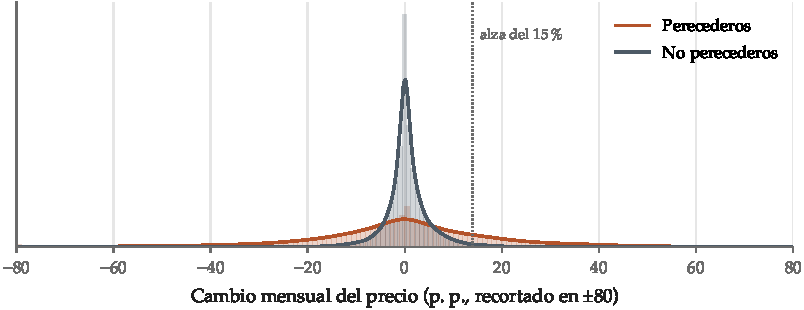
\includegraphics[width=.8\textwidth]{fig_distribucion}
\caption{Distribución del cambio mensual del precio para productos perecederos (frutas, verduras y tubérculos) y no perecederos: histograma y densidad estimada. La línea punteada marca un alza del 15\pct.}\label{fig:distribucion}
\end{figure}

\begin{figure}[htbp]\centering
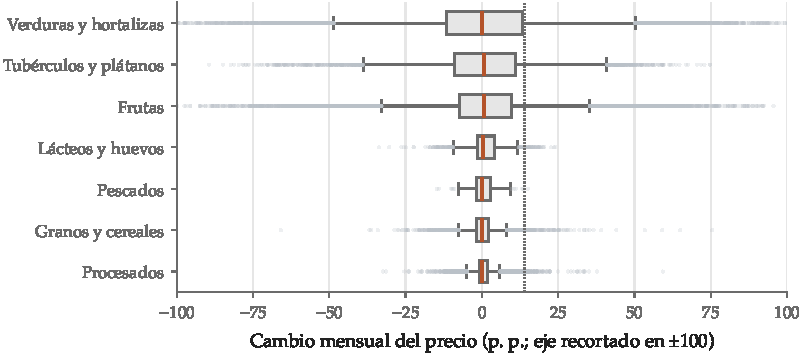
\includegraphics[width=.8\textwidth]{fig_cajas}
\caption{Diagrama de cajas del cambio mensual del precio por grupo de alimentos. La caja va del primer al tercer cuartil y la línea naranja es la mediana; la línea punteada marca un alza del 15\pct.}\label{fig:cajas}
\end{figure}

También hay diferencias importantes entre productos de un mismo grupo (tabla~\ref{tab:volatiles}). El mango Tommy y el limón Tahití registran alzas superiores al 15\pct\ en cerca de cuatro de cada diez meses, mientras que la leche en polvo, la sal y las pastas casi no presentan alzas de esa magnitud.

\begin{table}[htbp]\centering\small
\caption{Los diez productos con mayor y menor cambio mensual típico (mediana del cambio absoluto, p.~p.) y su porcentaje de alzas mayores al 15\,\%, entre los 82 productos con al menos 300 observaciones}\label{tab:volatiles}
\begin{adjustbox}{max width=\textwidth}\begin{tabular}{lrrlrr}\toprule
\multicolumn{3}{c}{Más volátiles} & \multicolumn{3}{c}{Menos volátiles}\\ \cmidrule(lr){1-3}\cmidrule(lr){4-6}
Producto & Cambio & Alzas & Producto & Cambio & Alzas\\ \midrule
Mango Tommy & 27{,}0 & 42 & Leche en polvo & 0{,}5 & 1 \\
Limón Tahití & 26{,}5 & 38 & Sal yodada & 0{,}9 & 1 \\
Pepino cohombro & 23{,}1 & 34 & Pastas alimenticias & 0{,}9 & 0 \\
Cilantro & 20{,}5 & 32 & Sardinas en lata & 1{,}0 & 1 \\
Mango común & 19{,}4 & 33 & Harinas & 1{,}3 & 1 \\
Limón común & 19{,}3 & 33 & Arroz & 1{,}5 & 1 \\
Habichuela & 19{,}2 & 34 & Lenteja & 1{,}9 & 2 \\
Tangelo & 17{,}3 & 30 & Azúcar & 2{,}1 & 3 \\
Mandarina Oneco & 16{,}7 & 29 & Maíz Blanco & 2{,}1 & 2 \\
Pepino de rellenar & 15{,}8 & 29 & Panela & 2{,}4 & 2 \\
\bottomrule\end{tabular}\end{adjustbox}\end{table}


\subsection*{Evolución en el tiempo}

Entre 2019 y 2026 el precio de frutas y tubérculos se duplicó, con un aumento generalizado en 2021 y 2022 (figura~\ref{fig:tiempo}a). La tasa mensual de alzas osciló entre el 8\pct\ y el 36\pct\ (figura~\ref{fig:tiempo}b), con un máximo en mayo de 2021 que coincide con los bloqueos de vías durante el paro nacional.

\begin{figure}[htbp]\centering
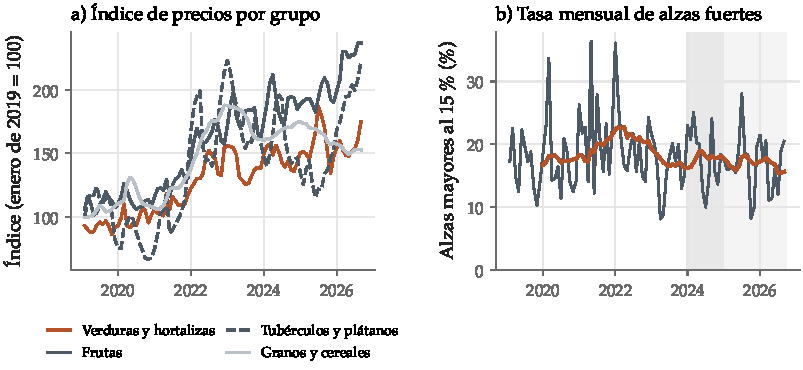
\includegraphics[width=.8\textwidth]{fig_tiempo}
\caption{(a) Índice de precios por grupo, construido encadenando el cambio logarítmico medio de las series de cada grupo. (b) Porcentaje de observaciones con alza mayor al 15\pct\ por mes pronosticado y su promedio móvil de doce meses; sombreado oscuro, validación; claro, prueba.}\label{fig:tiempo}
\end{figure}

En la figura~\ref{fig:anos} se observa que la dispersión del cambio en los perecederos fue estable hasta 2025 y disminuyó en 2026, y que las alzas fueron más frecuentes en 2021 y 2022. Como 2026 solo tiene datos hasta septiembre, la comparación se hizo con los mismos meses (enero a septiembre) de cada año: la desviación típica del cambio en los perecederos osciló entre \rvsdmin\ y \rvsdmax\ puntos de 2019 a 2024, fue de \rvsdveinticinco\ en 2025 y bajó a \rvsdveintiseis\ en 2026. La prueba de Kolmogorov--Smirnov entre desarrollo y prueba, con los mismos meses, rechaza la igualdad de distribuciones en frutas, verduras y granos, aunque con estadísticos pequeños (\rvksfru, \rvksver\ y \rvksgra), que reflejan sobre todo una dispersión menor en la prueba (por ejemplo, de \rvsdfrudes\ a \rvsdfrupru\ puntos en frutas). Un clasificador que intenta distinguir las observaciones de desarrollo y de prueba solo con el cambio del mes siguiente obtiene un AUC de \rvadvy, cercano a 0,5. La prueba es, por tanto, un periodo algo más tranquilo, con la misma forma de distribución.

\begin{figure}[htbp]\centering
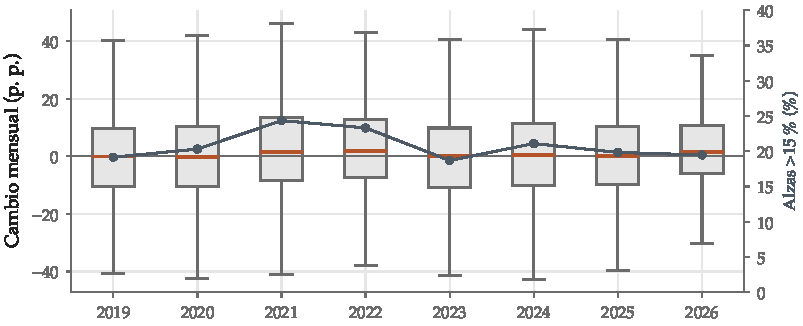
\includegraphics[width=.8\textwidth]{fig_anos}
\caption{Cambio mensual del precio de los productos perecederos por año: diagrama de cajas (sin valores extremos) y porcentaje de alzas mayores al 15\pct\ (línea, eje derecho).}\label{fig:anos}
\end{figure}

\subsection*{Estacionalidad}

La frecuencia de alzas varía según el mes del año y el grupo de alimentos. En verduras las alzas se concentran en diciembre y enero, en tubérculos en marzo y en frutas entre enero y marzo.


A nivel de producto el patrón estacional es aún más definido (figura~\ref{fig:estacional_productos}). La habichuela presenta alzas fuertes en el 72\pct\ de los eneros y la lechuga Batavia en el 65\pct\ de los diciembres, mientras que en otros meses estas alzas son poco frecuentes. Esta heterogeneidad motivó el cálculo de las variables estacionales para cada serie y no solo por grupo.

\begin{figure}[htbp]\centering
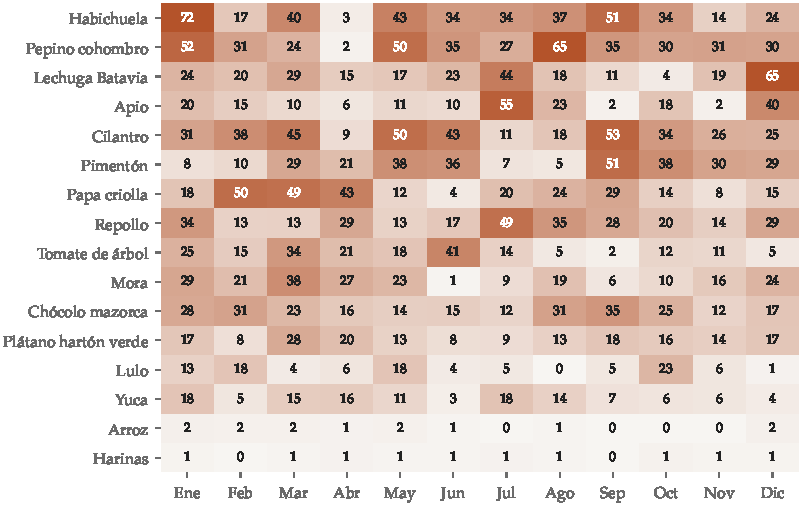
\includegraphics[width=.8\textwidth]{fig_estacional_productos}
\caption{Porcentaje de meses con alza mayor al 15\pct\ por producto y mes del año, para los 16 productos con más observaciones.}\label{fig:estacional_productos}
\end{figure}

\subsection*{Persistencia y autocorrelación}

Los movimientos fuertes tienden a agruparse en el tiempo. En la muestra de entrenamiento, después de un alza mayor al 15\pct\ la probabilidad de una nueva alza fuerte es del 29\pct, aproximadamente el doble que después de un mes sin movimientos grandes (15\pct); de forma simétrica, después de una baja mayor al 15\pct\ la probabilidad de otra baja fuerte es del 28\pct, frente al 12\pct\ después de un mes sin movimientos grandes.

La autocorrelación mediana del cambio mensual es \cacfuno\ en el primer rezago, \cacfdos\ en el segundo y \cacfdoce\ en el rezago doce (figura~\ref{fig:autocorrelacion}a). Este patrón es consistente con choques de oferta de corta duración que se revierten en los meses siguientes, junto con un componente estacional anual. El efecto de promediar las cotizaciones del mes (sección~\ref{sec:economia}) por sí solo produciría una autocorrelación de primer orden cercana a 0,25 si el precio diario siguiera un paseo aleatorio \citep{working1960}; que la observada sea menor indica que, además de ese efecto, parte de los choques se revierte de un mes a otro.

\begin{figure}[htbp]\centering
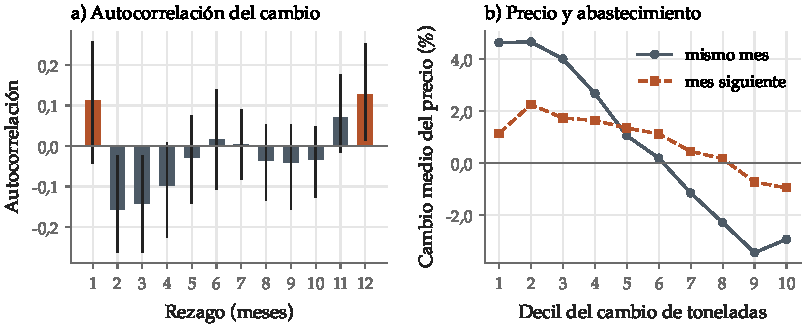
\includegraphics[width=.8\textwidth]{fig_autocorrelacion}
\caption{(a) Autocorrelación del cambio mensual del precio por rezago: mediana entre series y rango intercuartil. (b) Cambio medio del precio en el mismo mes y en el mes siguiente, por decil del cambio de las toneladas que entran a la central.}\label{fig:autocorrelacion}
\end{figure}

El mango Tommy de la Central Mayorista de Antioquia ilustra una serie con estacionalidad fuerte. La descomposición STL \citep{cleveland1990} muestra un ciclo anual con dos picos y una tendencia creciente desde 2021 (figura~\ref{fig:stl}). La fuerza estacional, $F_S=\max\{0,\,1-\operatorname{Var}(R_t)/\operatorname{Var}(S_t+R_t)\}$, con $S_t$ el componente estacional y $R_t$ el residuo \citep{wang2006,fpp3}, es de cerca de 0,8. En consecuencia, la autocorrelación del cambio mensual es alta en los rezagos 6 y 12 (0,44 y 0,56), y también en el rezago 24 (figura~\ref{fig:acf_ejemplo}).

\begin{figure}[htbp]\centering
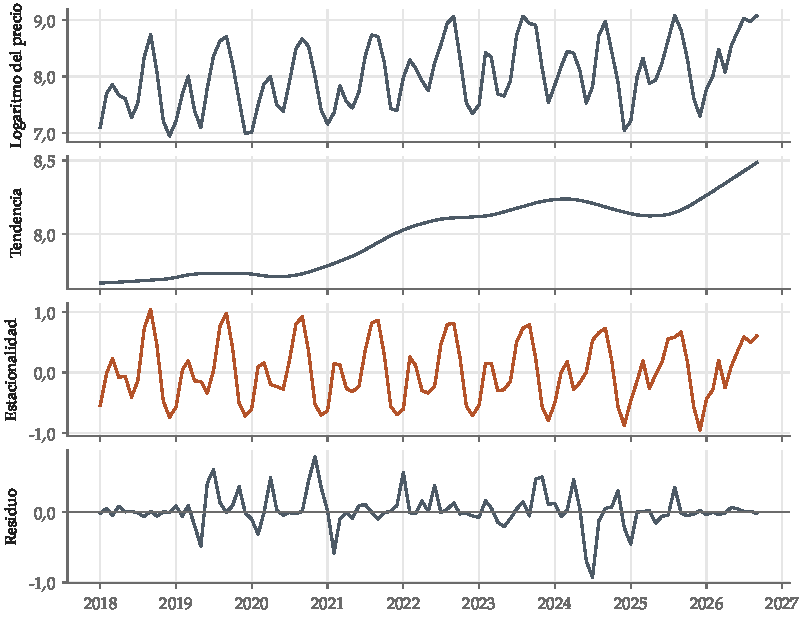
\includegraphics[width=.8\textwidth]{fig_stl}
\caption{Descomposición STL del logaritmo del precio del mango Tommy en la Central Mayorista de Antioquia, 2018--2026: serie, tendencia, estacionalidad y residuo.}\label{fig:stl}
\end{figure}

\begin{figure}[htbp]\centering
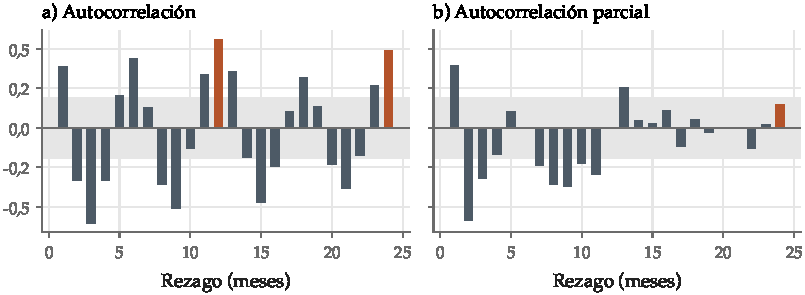
\includegraphics[width=.8\textwidth]{fig_acf_ejemplo}
\caption{Autocorrelación (a) y autocorrelación parcial (b) del cambio mensual del precio del mango Tommy en la Central Mayorista de Antioquia, con banda de no significancia al 95\pct. En naranja, los rezagos 12 y 24.}\label{fig:acf_ejemplo}
\end{figure}

\subsection*{Estacionariedad}

Con la prueba de Dickey--Fuller aumentada \citep{dickey1979} no se rechaza la hipótesis de raíz unitaria en el logaritmo del precio en el \rvadfno\pct\ de las series, mientras que para el cambio mensual se rechaza en casi todas (tabla~\ref{tab:adf}). No rechazar no prueba que exista raíz unitaria, y con unas 84 observaciones por serie la prueba tiene poca potencia. Por eso se complementó con la prueba KPSS \citep{kpss1992}, cuya hipótesis nula es la estacionariedad: esta rechaza en el \rvkpssrech\pct\ de las series, ambas pruebas indican raíz unitaria en el \rvkpssambas\pct\ y ambas indican estacionariedad alrededor de una tendencia en el \rvkpssest\pct. Las pruebas no se ajustaron por multiplicidad, de modo que estas proporciones son descriptivas. La evidencia de raíz unitaria es, entonces, mixta en el nivel y clara a favor de la estacionariedad en el cambio, lo que respalda modelar el cambio del precio.

\begin{table}[htbp]\centering\small
\caption{Pruebas de raíz unitaria (Dickey--Fuller aumentada, $H_0$: raíz unitaria) y de estacionariedad (KPSS, $H_0$: estacionariedad) en las 1.230 series con al menos cinco años de datos, al 5\,\% y sin ajuste por multiplicidad}\label{tab:adf}
\begin{adjustbox}{max width=\textwidth}\begin{tabular}{llr}\toprule
Serie y prueba & Componentes & Series (\%)\\ \midrule
\multicolumn{3}{l}{\emph{Logaritmo del precio}}\\
\quad ADF: no rechaza la raíz unitaria & constante y tendencia & 51{,}5 \\
\quad KPSS: rechaza la estacionariedad & constante y tendencia & 34{,}9 \\
\quad Ambas indican raíz unitaria & & 26{,}6 \\
\quad Ambas indican estacionariedad alrededor de una tendencia & & 40{,}2 \\
\multicolumn{3}{l}{\emph{Cambio mensual}}\\
\quad ADF: rechaza la raíz unitaria & constante & 95{,}7 \\
\quad KPSS: rechaza la estacionariedad & constante & 0{,}7 \\
\bottomrule\end{tabular}\end{adjustbox}\end{table}


\section{Las variables explicativas}
\label{sec:explicativas}

A partir del precio, el abastecimiento y el ONI se construyeron 52 variables candidatas (tabla~\ref{tab:bloques}), cuya definición operativa está en la tabla~\ref{tab:variables} del apéndice. La tabla~\ref{tab:explicativas} resume las principales en la muestra de entrenamiento. Salvo las de abastecimiento, presentan muy pocos faltantes. Su relación individual con el cambio del mes siguiente es débil, con una correlación máxima de 0,27 en valor absoluto, de modo que cualquier ganancia de los modelos dependerá de la combinación de varias variables.

\begin{table}[htbp]\centering\small
\caption{Variables explicativas principales en entrenamiento: porcentaje de faltantes, mediana, cuartiles y correlación de Spearman con el cambio del mes siguiente}\label{tab:explicativas}
\begin{adjustbox}{max width=\textwidth}\begin{tabular}{llrrrrr}\toprule
Variable & Unidad & Faltantes (\%) & Mediana & Q1 & Q3 & $\rho_S$ con $y$\\ \midrule
Cambio del precio, 1 mes & p. p. & 0{,}3 & 0{,}4 & \ensuremath{-}7{,}5 & 9{,}6 & 0{,}101 \\
Cambio del precio, 12 meses & p. p. & 0{,}0 & 10{,}4 & \ensuremath{-}6{,}2 & 28{,}8 & \ensuremath{-}0{,}138 \\
Volatilidad 12 meses & p. p. & 0{,}9 & 15{,}6 & 8{,}9 & 23{,}4 & \ensuremath{-}0{,}004 \\
Distancia al máximo anual & p. p. & 0{,}3 & \ensuremath{-}16{,}9 & \ensuremath{-}39{,}2 & \ensuremath{-}2{,}5 & \ensuremath{-}0{,}182 \\
Frecuencia histórica de alzas en el mes & \% & 0{,}0 & 11{,}0 & 4{,}2 & 25{,}0 & 0{,}183 \\
Cambio histórico en el mes & p. p. & 0{,}0 & 0{,}4 & \ensuremath{-}5{,}4 & 6{,}8 & 0{,}270 \\
Cambio en las demás centrales, 1 mes & p. p. & 0{,}0 & 0{,}7 & \ensuremath{-}5{,}6 & 7{,}5 & 0{,}160 \\
Demás centrales con alza en t & \% & 0{,}0 & 5{,}3 & 0{,}0 & 26{,}1 & 0{,}117 \\
Cambio de toneladas, 1 mes & p. p. & 1{,}6 & 0{,}2 & \ensuremath{-}20{,}5 & 21{,}3 & \ensuremath{-}0{,}051 \\
ONI & \textdegree C & 0{,}0 & \ensuremath{-}0{,}3 & \ensuremath{-}0{,}8 & 0{,}6 & \ensuremath{-}0{,}067 \\
\bottomrule\end{tabular}\end{adjustbox}\end{table}


\subsection*{Abastecimiento}

Las toneladas que ingresan a las centrales muestran un crecimiento gradual y una estacionalidad moderada (figura~\ref{fig:abastecimiento}a). Un mayor volumen se asocia con una leve disminución del precio en el mismo mes (correlación mediana de $-0{,}11$), pero la relación con el precio del mes siguiente es prácticamente nula (figuras~\ref{fig:abastecimiento}b y~\ref{fig:autocorrelacion}b).

\subsection*{Transmisión entre centrales}

El precio del mismo producto en otras centrales presenta la asociación más fuerte con el cambio del precio (figura~\ref{fig:abastecimiento}b). La asociación contemporánea es fuerte (correlación mediana de 0,73) y la adelantada es débil: la correlación mediana con el cambio de las demás centrales en el mes anterior es de 0,20. Esta señal adelantada podría reflejar la autocorrelación del propio precio o el efecto de promediar (sección~\ref{sec:economia}). Sin embargo, en la muestra de entrenamiento la correlación entre el cambio del mes siguiente y el cambio de las demás centrales en el mes actual es de \rvwknac, y controlando por el cambio propio del mes actual baja solo a \rvwkparcial; el cambio propio, en cambio, tiene una correlación de \rvwkpropio. La señal de las demás centrales no se explica, entonces, por la autocorrelación propia.

\begin{figure}[htbp]\centering
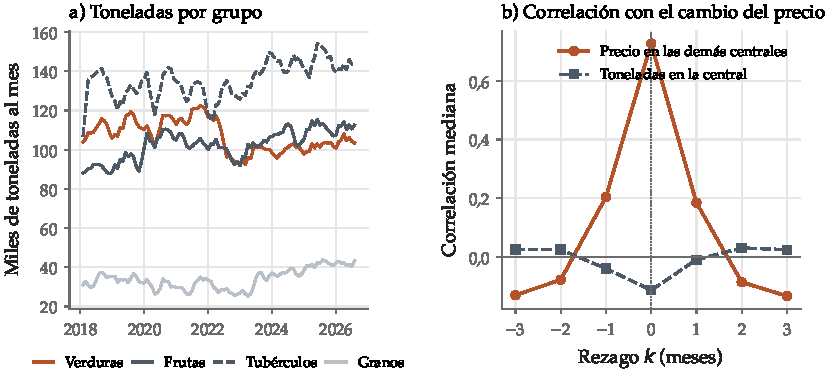
\includegraphics[width=.8\textwidth]{fig_abastecimiento}
\caption{(a) Toneladas mensuales que entran a las centrales del panel por grupo (media móvil de tres meses). (b) Correlación mediana entre series del cambio del precio en el mes $t$ con el cambio en el mes $t+k$ del precio en las demás centrales y de las toneladas en la propia central; $k<0$ indica que la variable va antes que el precio.}\label{fig:abastecimiento}
\end{figure}

\subsection*{El Niño}

Según la serie del ONI usada \citep{noaa} y la clasificación habitual por el valor máximo (débil, de 0,5 a 0,9; moderado, de 1,0 a 1,4; fuerte, de 1,5 a 1,9; muy fuerte, 2,0 o más), entre 2018 y 2026 hubo un episodio moderado de El Niño (2018--2019), uno débil (2019--2020), uno muy fuerte (2023--2024) y otro que comenzó en 2026, además de un periodo prolongado de La Niña entre 2020 y comienzos de 2023. La correlación entre el ONI y la tasa de alzas es cercana a cero para rezagos entre cero y seis meses. Este resultado no excluye efectos del clima a escala regional \citep{bohorquez2026}, pero indica que el índice agregado tiene poca utilidad para pronosticar el mes siguiente.


\subsection*{Correlaciones entre variables}

En la figura~\ref{fig:correlaciones} se observan tres grupos de variables asociadas con el cambio futuro. Las variables estacionales se correlacionan positivamente con él; la posición del precio respecto a su máximo y mínimo del último año se correlaciona negativamente, y el cambio en las demás centrales, positivamente. Algunas variables explicativas están muy correlacionadas entre sí, lo cual se tuvo en cuenta en la selección de variables.

\begin{figure}[htbp]\centering
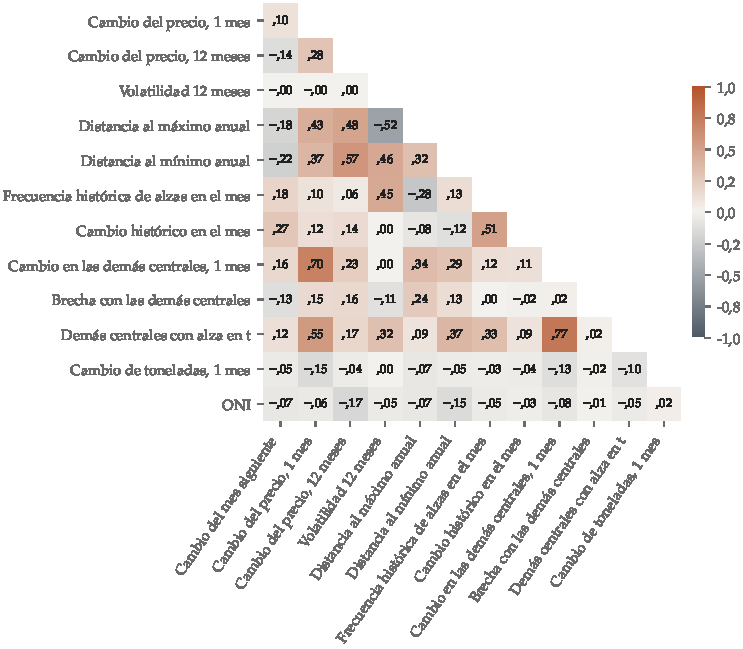
\includegraphics[width=.8\textwidth]{fig_correlaciones}
\caption{Correlaciones de Spearman entre el cambio del mes siguiente y las variables explicativas principales, en la muestra de entrenamiento.}\label{fig:correlaciones}
\end{figure}

\FloatBarrier
\section{Conclusiones del análisis exploratorio}
\label{sec:conclusiones_eda}

Los datos del SIPSA presentan una calidad adecuada para el estudio. Falta el \cfaltserie\pct\ de los precios, en su mayoría en huecos de uno o dos meses, y se identificó un solo error de registro. En el nivel del precio la evidencia de raíz unitaria es mixta, mientras que el cambio mensual es estacionario en casi todas las series, por lo que se modeló el cambio; la presencia de colas pesadas justifica el uso de la pérdida absoluta. Los movimientos grandes se concentran en los productos perecederos, lo que anticipa una capacidad de pronóstico desigual entre grupos. La estacionalidad es marcada y específica de cada producto, por lo que se calcularon variables estacionales por serie. Los movimientos fuertes tienden a agruparse en el tiempo, y el cambio del precio tiene una asociación contemporánea fuerte con el de las demás centrales y una señal adelantada débil. En cambio, ni el abastecimiento de la propia central ni el ONI mostraron relación con el cambio del mes siguiente.

\FloatBarrier
